\documentclass{tudscrartcl}
\usepackage[ngerman]{babel}
\usepackage{textcomp}
\usepackage{standalone}[subpreambles=false]
\usepackage{tikz}
\usepackage{amsmath}
\usepackage{nicefrac}
\usepackage{mathtools}
\usepackage[locale=DE]{siunitx}
\usepackage{graphicx}
\usetikzlibrary{shapes,arrows,positioning}
\graphicspath{{./Images/}}


\title{Control}
\author{James Vero Asghar}

\begin{document}
    \pagenumbering{gobble}
    \maketitle
    \newpage
    \pagenumbering{arabic}

\section{Analyse der Aufgabenstellung}
        
\subsection{Motivation, Aufgabenstellung / Ziel des Semesters}

In diesem Seminar muss einen Roboter einen Parcour umfahren, eine Parklücke erkennen, darin einparken und dann ausparken. Dieses Seminar ist eine kleine Version des aktuellen Technikproblems von autonomem Fahren. Der Parcour ist im Abbildung \ref{fig:map} zu sehen. \\

\begin{figure}
    \centering
    
\includegraphics{map}
    \caption{Parcour}
    \label{fig:map}
\end{figure}

Das Seminarprojekt besteht aus f"unf Modulen, die jeweils von einem Gruppenmitglied bearbeitet werden. Die Module sind Guidance, Control, Navigation, Perception und Human-Machine-Interface (HMI). Guidance koordiniert die andere vier Modulen, sodass der Roboter sein Ziel erreichen kann. Control steuert die Bewegung des Roboters. Navigation stellt die aktuelle Position des Roboters fest und identifiziert die Parklücke. Perception k"ummert sich um die Messfehler der Sensoren und berechnet, wie pr"asizese sie sind. HMI erstellt eine Android-App, um ein Interface mit dem Roboter zu haben, sodass ein Benutzer dem Roboter Kommandos geben kann. \\

Die f"unf Module arbeiten eng zusammen. Zum Beispiel muss Navigation mit Perception arbeiten, sodass der Roboter die Messfehler der Sensoren ausgleichen kann, um eine richtige aktuelle Position zu berechnen. Diese Beziehung zwischen den Modulen ist "ahnlich wie bei einer reellen Anwendung, weil ein Projekt normalerweise nicht durch nur eine Person erarbeitet werden kann. Stattdessen m"ussen viele Aufgaben parallel abgeschlossen werden, um das Projekt abzuschlie"sen. \\

Der Fokus dieser Seminararbeit sind das Control-Modul und alle Teilaufgaben, die dazu geh"oren. \\

\subsection{Zusammenfassung der einzelnen Teilaufgaben}

Das Control-Modul hat vier Teilaufgaben: Linieverfolgung, \(v/\omega\)-Control, geregeltes Geradeausfahren und Ein-/Ausparken. \\

F"ur die Linienverfolgung muss der Roboter mit zwei Lichtsensoren einer schwarzen Linie schnellstm"oglichst folgen und um die Ecken des Parcours navigieren. \\

F"ur die \(v/\omega\)-Control muss eine Methode implementiert werden, sodass der Roboter mit einer konstanten Geschwindigkeit und Drehgeschwindigkeit fahren kann. Mit dieser Methode soll der Roboter einfache Kreise, Ellipsen, und f"ur kurze Strecken gerade ausfahren k"onnen. \\

Die dritte Teilaufgabe ist die Verbesserung des Geradeausfahrens. Der Roboter muss nun f"ur lange Strecken gerade ausfahren. \\

Die vierte und letzte Teilaufgabe ist die Entwicklung eines Algorithmus f"ur das Ein-/Ausparken des Roboters. Diese Aufgabe muss in enger Zussamenarbeit mit dem Guidance-Modul abgeschlossen werden. Das Guidance-Modul liefert Control die Information, wohin der Roboter fahren muss. Control implementiert einen Algorithmus, sodass der Roboter diese Information in eine Bahn "ubersetzt kann.

\subsection{\"Ubergabeparameter von / zu Control-Modul}

Das Control-Modul ist das Herz des Roboters. Ohne das Control-Modul kann der Roboter sich nicht bewegen und es braucht im Vergleich zu den anderen Modulen die meistene Parameter. F"ur die Linienverfolgung braucht Control die Werte der Lichtsensoren von Perception und f"ur \(v/\omega\)-Control braucht Control die Werte der beiden Motorenencoder, sodass eine sinnvolle Regelung implementiert wird. F"ur die Geradeausfahrt wird die aktuelle Position gebraucht, die von Navigation berechnet wird. Das Ein-/Ausparken ben"otigt die Parkbahn von Guidance. Die Parkbahn ist abh"angig von dem implementierten Algorithmus und kann auf entweder Zielpunkten oder Polynomen basieren.


\section{Linienverfolgung}
    \subsection{Verbesserung des Beispielprogrammes}

Das Beispielprogramm bekommt die diskrete Werte 0, 1, und 2 von Perception, um zu verstehen, ob ein Lichtsensor auf eine schwarze oder weisse Linie ist. Der Roboter ver"andern seine Motoren zwischen zwei PWM-Werten abh"angig von den diskreten Werten, sodass er immer um die Linie oscilliert. \\

Die Schwingungen um die schwarze Linie sind unerw"unscht. Um die Schwingungen zu unterdr"ucken muss der Differenz zwischen den beiden PWM-Werten verkleinert werden. Die PWM-Werten d"urfen auch nicht zu hoch sein oder der Roboter kann die Ecken des Parcours nicht navigieren.

\subsection{Einf\"uhrung eines PID-Reglers}

\begin{figure}
    \centering
    % Title: Block diagram of Third order noise shaper in Compact Disc Players
% Author: Ramón Jaramillo
\documentclass{standalone}
\usepackage{babel}
\usepackage{german}
\usepackage{textcomp}
\usepackage{tikz}
\usetikzlibrary{shapes,arrows}
\begin{document}
% Definition of blocks:
\tikzset{
block/.style    = {draw, thick, rectangle, minimum height = 3em,
  minimum width = 3em},
sum/.style      = {draw, circle, node distance = 2cm, inner sep = 0pt,
minimum size = 0.5cm}, % Adder
input/.style    = {coordinate}, % Input
output/.style   = {coordinate} % Output
}
% Defining string as labels of certain blocks.
\newcommand{\suma}{\Large$+$}
\newcommand{\inte}{$\displaystyle \int$}
\newcommand{\derv}{\huge$\frac{d}{dt}$}
\begin{tikzpicture}[auto, thick, node distance=2.25cm, >=triangle 45]
\draw
% Drawing the blocks of first filter :
    node at (0,0) [right=0mm]{}
    node [input] (input1) {} 
    node [sum, right of=input1] (suma1) {\suma}
    node [right of=suma1] (branch1) {}
    node [block, right of=branch1] (Ki) {$\displaystyle Ki\cdot\int_{0}^{t} e(t)\, dt$}
    node [block, above of=Ki] (Kp) {$Kp \cdot e(t)$}
    node [block, below of=Ki] (Kd) {$Kd\cdot\frac{d}{dt} e(t)$}
    node [sum, right of=Ki] (suma2) {\suma}
    node [block, right of=suma2] (plant) {Regelstrecke}
    node [right of=plant] (branch2) {}
    node [output, right of=branch2] (output1) {}
    node [below of=Kd] (branch3) {}
;

% Joining blocks. 
% Commands \draw with options like [->] must be written individually
\draw[->] (input1) -- node {$x(t)$} (suma1);
\draw[-] (suma1) -- node {$e(t)$} (branch1.center);
\draw[->] (branch1.center) -- (Ki);
\draw[->] (branch1.center) |- (Kp);
\draw[->] (branch1.center) |- (Kd);
\draw[->] (Ki) -- (suma2);
\draw[->] (Kp) -| (suma2);
\draw[->] (Kd) -| (suma2);
\draw[-] (suma2) -- node {\(u(t)\)} (plant);
\draw[-] (plant) -- (branch2.center);
\draw[-] (branch2.center) |- (branch3.center);
\draw[->] (branch2.center) -- node {$y(t)$} (output1);
\draw[->] (branch3.center) -| node[pos=0.97, xshift=-5] {\huge $-$} (suma1);

\filldraw
    (branch1) circle (2pt)
    (branch2) circle (2pt)
;
\end{tikzpicture}
\end{document}
    \caption{Regelkreis}
    \label{fig:regelkreis}
\end{figure}

Nun wird nur eine Regelgr"o"se \(y(t)\) betrachtet. Die ist der Differenz zwischen den linken und rechten Lichtintensit"aten der Lichtsensoren.
\begin{equation}
    Lichtintensit"at_L - Lichtintensit"at_R = Regelgr"o"se \: y(t)
\end{equation}

 Der Bereich der Regelgr"o"se liegt zwischen \si{-100\percent} und \si{100\percent}. Die zwei Werte bedeuten, dass bei -100\% der rechte Lichtsensor auf weiss liegt und der linke Lichtsensor auf schwarz liegt und bei \si{100\percent} das Gegenteil. Die F"uhrungsgr"o"se \(x(t)\) ist \si{0\percent}, weil dabei beiden Lichtsensoren auf weiss liegen. Der Regelfehler \(e(t)\) ist unver"andert. Es gibt nur ein Tupel von PID-Konstanten \({Kp,Ki,Kd}\) und deshalb ist nur ein Regelkreis ben"otigt, der nochmal in Abbildung \ref{fig:regelkreis} zu sehen ist. Bevor die Ausgabe des Reglers direkt in den Motoren geschickt werden kann, muss zuerst das Vorzeichen von der rechten Motoreingabe umgekehrt werden. Falls die beiden Eingabe der Motoren positiv w"aren, f"uhrt der Regelkreis zu einer Mitkopplung auf dem rechten Motor statt Gegenkopplung. Dieses liegt an dem ver"andernten Bereich der Regelgr"o"se, weil der nun negative Werte besitzt. Negative Werte bedeuten eine rechte Ablenkung, deshalb muss der rechte Motor einen positiven PWM-Wert bekommen und der linke Motor das Gegenteil, um diese Ablenkung zu kompensieren. \\

Diese Methode funktioniert mit wenigen Problemen und der Roboter verfolgt die Linie mit den folgenden PID-Konstanten 
\begin{equation*}
    \left(Kp, Ki, Kd\right) = \left(\num{0.4}, \num{0.2}, \num{0.0565}\right).
\end{equation*}
Manchmal "uberspringt der Roboter eine Ecke und l"auft der Roboter in einem Kreis, ohne die Linie wieder zu erkennen. Dieses Verhalten passiert selten, aber scheint es darauf, haupts"achlich die Konversion zwischen Gleitkommazahlen und Integerzahlen. Der Regler gibt Gleitkommazahlen aus, aber die Motoren brauchen Integerwerten. Deswegen muss der Roboter die Ausgabe des Reglers von Double zu Integer typecasten. Das Typecasten f"uhrt zu Ungenauigkeiten in den PWM-Werten, deswegen w"urde der Roboter zu weit ablenken und weg von der Linie fahren.

\section{\(v/\omega\)-Control}
    \subsection{Steuerung}

Konnte einfache Kreise am Platz machen, gibt immer eine Abweichung mit der Ellipse und Geradeausfahrt\\

Der Roboter muss jetzt mit einer bestimmten Geschwindigkeit \(v\) und Winkelgeschwindigkeit \(\omega\) fahren. Zuerst muss die Kinematik des Roboters berechnet werden. Gegeben ist die kinematischen Matrix, die die Geschwindigkeiten der R"adern \(v_l, v_r\) zu der Geschwindigkeit des Achsmittelpunktes \(v_m\) und der Winkelgeschwindigkeit \(\omega\) verbinden,
\begin{equation}
    \begin{pmatrix}
        v_m \\
        \omega
    \end{pmatrix}
    =
    \begin{pmatrix}
        \nicefrac{1}{2} & \nicefrac{1}{2} \\
        \nicefrac{1}{-d} & \nicefrac{1}{d}
    \end{pmatrix}
    \begin{pmatrix}
        v_l \\
        v_r
    \end{pmatrix}
\end{equation}
mit \(d\) als die Achsenl"ange. 
Davon ist die inverse Matrix berechnet, sodass \(v_l\) und \(v_r\) von \(v_m\) und \(\omega\) ausgerechnet werden k"onnen:
\begin{equation}
    \begin{pmatrix}
        v_l \\
        v_r
    \end{pmatrix}
    = 
    \begin{pmatrix}
        1 & \nicefrac{-d}{2} \\
        1 & \nicefrac{d}{2}
    \end{pmatrix}
    \begin{pmatrix}
        v_m \\
        \omega
    \end{pmatrix}
    .
\end{equation} \\

Als n"achstes muss die Drehzahl den beiden R"adern berechnet werden. Das ist erfolgreich durch die folgende Gleichung:
\begin{equation}
    \omega_{l,r} = \dfrac{v_{l,r}}{R_{l,r}},
\end{equation}
mit \(R_{l,r}\) als die Radien der linken und rechten R"adern. \\

Letzlich muss die PWM-Werte \(u_{PWM,l,r}\) der Motoren berechnet werden. Obwohl der Zussamenhang zwischen die Drehzahlen \(\omega_{l,r}\) und die PWM-Werte nicht linear ist, d"urfte der Roboter dieser Zusammenhang als eine lineare Gleichung im Form von
\begin{equation}
    u_{PWM,l,r} = k_{m,l,r} \, \omega_{l,r} + u_{PWM,Y-Schnittpunkt,l,r}
\end{equation}
approximieren, weil der PWM-Wert von dem Y-Schnittpunkt linear steigt. \\

Die Motorenkonstanten \(k_{m,l,r}\) und PWM-Y-Schnittpunkten \(u_{PWM,Y-Schnittpunkt,l,r}\) werden experimentell bestimmt. Ein Program l"auft auf dem Roboter, das die PWM-Werte der Motoren von \si{0\percent} bis \si{100\percent} mit einer Rate von \si{1 \volt_{PWM}\per\second} hochfährt. Jede Sekunde werden die PWM-Werte und Drehzahlen der Motoren aufgenommen. Die aufgenommenen Werte werden in einer Tabelle geschrieben und einem Diagramm dargestellt. Die Drehzahlen sind auf dem X-Achse und die PWM-Werte sind auf dem Y-Achse. Durch lineare Regression wird zwei lineare Funktionen zwischen den Drehzahlen und den PWM-Werten bestimmt. Davon sind die Steigungen der Funktionen die Motorenkonstanten und Y-Schnittpunkte sind die PWM-Y-Werte. Mit dieser Funktion ist die Kette von \(v_m\) und \(\omega\) zu \(u_{PWM,l,r}\) fertig. \\

Mit dieser Methode kann der Roboter einfache Kreise am Platz fahren, aber der Roboter kann nicht ohne Abweichungen gerade  ausfahren und Ellipse fahren. Das liegt darauf, dass diese Methode nur eine Steuerung ist und nicht eine Regelung. Bei Steuerung hat die Ausgabe keinen Einfluss auf der Eingabe. Deshalb hat der Regelkreis einer Steuerung keine Gegenkopplung von Ausgabe zu Eingabe. Der Regelkreis der \(v/\omega\)-Steuerung ist in Abbildung \ref{fig:steuerung} zu sehen. Ohne dieser R"uckf"uhrung kann der Roboter nicht wissen wie schnell der f"ahrt. \\

\begin{figure}
    \centering
    \documentclass{standalone}
\usepackage{babel}
\usepackage{german}
\usepackage{textcomp}
\usepackage{tikz}
\usepackage{mathtools}
\usepackage{nicefrac}
\usetikzlibrary{shapes,arrows,positioning}
\begin{document}
\tikzset{
block/.style    = {draw, thick, rectangle, minimum height = 3em,
  minimum width = 3em},
sum/.style      = {draw, circle, node distance = 2cm, inner sep = 0pt,
minimum size = 0.5cm}, % Adder
input/.style    = {coordinate}, % Input
output/.style   = {coordinate} % Output
}
\newcommand{\suma}{\Large$+$}
\newcommand{\inte}{$\displaystyle \int$}
\newcommand{\derv}{\huge$\frac{d}{dt}$}
\begin{tikzpicture}[auto, thick, node distance=2cm, >=triangle 45]
\node [block] (matrix) {\(
        \begin{psmallmatrix}
            1 & \nicefrac{-d}{2} \\
            1 & \nicefrac{d}{2} 
        \end{psmallmatrix}
    \)}
;
\node [input, left=of matrix.160] (vm) {};
\node [input, left=of matrix.200] (w) {};

\node [block, right=of matrix] (radius) {\(\dfrac{1}{R_{l,r}}\)};
\node [input, right=of matrix.20] (vl) {\(v\)};
\node [input, right=of matrix.340] (vr) {\(\omega\)};

\node [block, right=of radius] (function) {Steuerung};
\node [input, right=of radius.30] (wl) {};
\node [input, right=of radius.330] (wr) {};

\node [input, right=of function.20] (ul) {};
\node [input, right=of function.340] (ur) {};

\draw[->] (vm) -- node {\(v_m\)} (matrix.160);
\draw[->] (w) -- node [below] {\(\omega\)} (matrix.200);

\draw[->] (matrix.20) -- node {\(v_l\)} (vl);
\draw[->] (matrix.340) -- node [below] {\(v_r\)} (vr);

\draw[->] (radius.30) -- node {\(\omega_l\)} (wl);
\draw[->] (radius.330) -- node [below] {\(\omega_r\)} (wr);

\draw[->] (function.20) -- node {\(u_{PWM,l}\)} (ul);
\draw[->] (function.340) -- node [below] {\(u_{PWM,r}\)} (ur);

\end{tikzpicture}
\end{document}
    \caption{\(v/\omega\)-Steuerung}
    \label{fig:steuerung}
\end{figure}


\subsection{Regelung}

Bei der Einführung eines Reglers ist das Verhalten des \(v/\omega\)-Steuerung viel genauerer. Der Regelkreis mit dem Regler ist in Abbildung 3 zu sehen. Aber am Anfang lief der Roboter nicht problemlos. Mit der ersten Version des Reglers fährt der Roboter ziemlich genau gerade mit einer pr"azisen Geschwindigkeit, aber der Roboter konnte nicht am Platz mit einer präzisen Drehgeschwindigkeit drehen. Der Roboter w"urde immer ein bisschen zu wenig drehen. Diese Problem lag an der Nichtlinearität des Motors. Jeder Motor hat eine bestimmte tote Zone oder in englischen “Deadzone”, die der Motor beseitigen muss, bevor er anfangen kann, zu drehen. Die tote Zone kommt von der inneren Reibung des Motors und muss bei jedem Regler berücksichtigt werden. \\

Eine Methode, um diese tote Zone zu kompensieren, ist durch die Implementation einer Steuerung. Weil der Roboter schon eine Steuerung hatte, konnte der Roboter gerade fahren. Aber mit nur dieser Steuerung konnte der Roboter problemlos drehen. Deswegen wird ein Arbeitspunkt zu dem Regler hinzufügt. \\

Die zweite Version des Reglers hat ein richtig präzise Führungsverhalten mit dem gerade Fahren und Drehen. Aber der Arbeitspunkt des Reglers liefert eine ziemlich hohe "Uberschwingung zu der Regelstrecke, die manchmal zwingt, der Roboter zu weit zu drehen. Die "Uberschwingung ist in Abbildung \ref{fig:vw-control} zu sehen. \\ 

\begin{figure}
    \centering
    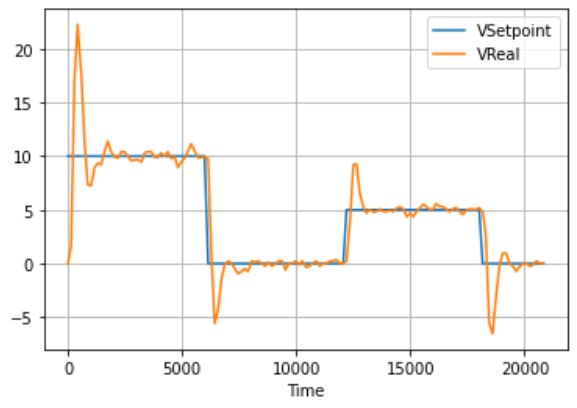
\includegraphics{vw-control}
    \caption{"Uberschwingung}
    \label{fig:vw-control}
\end{figure}

Die dritte Version des Reglers implementiert eine nichtlineare Funktion, um den Arbeitspunkt des Regler zu setzen. Bei niedriger Geschwindigkeit und Drehgeschwindigkeit wird der Arbeitspunkt hoch gesetzt, um die tote Zone zu kompensieren, und bei hoher Geschwindigkeit und Drehgeschwindigkeit wird er tiefer gesetzt. Die nichtlineare Funktion wird benötigt, weil der Arbeitspunkt plus Steuerung zusammen eine Überkompensation zu der Regelstrecke liefert. Deswegen wird der Arbeitspunkt tiefer, wenn er bei hoher Geschwindigkeit und Drehgeschwindigkeit nicht mehr benötigt ist. Der fertige Regelkreis ist in Abbildung \ref{fig:regelung} zu sehen. \\

\begin{figure}
    \centering
    % Title: Block diagram of Third order noise shaper in Compact Disc Players
% Author: Ramón Jaramillo
\documentclass{standalone}
\usepackage{babel}
\usepackage{german}
\usepackage{textcomp}
\usepackage{tikz}
\usetikzlibrary{shapes,arrows}
\begin{document}
% Definition of blocks:
\tikzset{
block/.style    = {draw, thick, rectangle, minimum height = 3em,
  minimum width = 3em},
sum/.style      = {draw, circle, node distance = 2cm, inner sep = 0pt,
minimum size = 0.5cm}, % Adder
input/.style    = {coordinate}, % Input
output/.style   = {coordinate} % Output
}
% Defining string as labels of certain blocks.
\newcommand{\suma}{\Large$+$}
\newcommand{\inte}{$\displaystyle \int$}
\newcommand{\derv}{\huge$\frac{d}{dt}$}
\begin{tikzpicture}[auto, thick, node distance=2.25cm, >=triangle 45]
\draw
% Drawing the blocks of first filter :
    node at (0,0) [right=0mm]{}
    node [input] (input1) {} 
    node [right of=input1] (branch1) {}
    node [sum, right of=branch1] (suma1) {\suma}
    node [block, above of=suma1] (steuerung) {Steuerung}
    node [block, right of=suma1] (PID) {PID}
    node [sum, right of=PID] (suma2) {\suma}
    node [block, right of=suma2] (plant) {Regelstrecke}
    node [right of=plant] (branch2) {}
    node [block, below of=suma2] (branch3) {Encoder}
;

% Joining blocks. 
% Commands \draw with options like [->] must be written individually
\draw[-] (input1) -- node {\(\omega_{l,r}\)} (branch1.center);
\draw[->] (branch1.center) -- (suma1);
\draw[-] (branch1.center) |- (steuerung);
\draw[->] (steuerung) -| (suma2);
\draw[-] (suma1) -- (PID);
\draw[->] (PID) -- (suma2);
\draw[-] (suma2) -- (plant);
\draw[-] (plant) -- (branch2.center);
\draw[-] (branch2.center) |- (branch3);
\draw[->] (branch3) -| node[pos=0.30, label={\(\omega_{Real,l,r}\)}] {} node[pos=0.97, xshift=-5] {\huge $-$} (suma1);

\filldraw
  (branch1) circle (2pt)
;
\end{tikzpicture}
\end{document}
    \caption{\(v/\omega\)-Regelung}
    \label{fig:regelung}
\end{figure}

Die Implementierung der dritten Version des Reglers auf dem Roboter erlaubt die pr"asizen Bewegungen von Kreisen und Ellipsen. Der Roboter kann auch f"ur ziemlich weite Strecken auch gerade fahren. Manchmal dreht er sich ein bisschen zu weit, aber das ist selten.



\section{Regelung der Geradeausfahrt}
    Die Implementation einer geregelten Geradeausfahrt eines Roboters braucht ein paar Schritte. Zuerst muss ein funktionierdes Modell des Roboters gefunden werden. Danach muss irgendeine Querabweichung ber"ucksichtigt werden. Am Ende kann ein Regler f"ur das System gefunden werden. 

\subsection{Linearisierung in $X_2$-Richtung}

Die folgende Modellgleichung eines einachsigen Roboters wird gegeben:
\begin{equation} \label{eq:model}
    \overrightarrow{f}(\overrightarrow{x}, \overrightarrow{u}) =
    \begin{bmatrix*}
        \dot{x}_1 \\
        \dot{x}_2 \\
        \dot{x}_3
    \end{bmatrix*}
    =
    \begin{bmatrix*}
        \sin(x_3) & 0 \\
        \cos(x_3) & 0 \\
        0 & 1
    \end{bmatrix*}
    \begin{bmatrix*}
        v \\
        \omega
    \end{bmatrix*}
\end{equation}.

Wegen des nichtlinearen Forms der Modellgleichung ist es schwierig das Systemverhalten des Modells zu beobachten. Deshalb wird sie in einem Arbeitspunkt linearisiert und dann wird dieses Modells betrachtet. Im Folge ist die Herleitung des linearisierten Modells:

\begin{equation}
    \overrightarrow{\widetilde{f}}(\overrightarrow{\widetilde{x}}, \overrightarrow{\widetilde{u}}) =
    \begin{bmatrix*}
        \dot{x}_1 \\
        \dot{x}_2 \\
        \dot{x}_3
    \end{bmatrix*}
    =
    \begin{bmatrix*}
        0 & 0 & \cos(x_{30})v_0 \\
        0 & 0 & -\sin(x_{30})v_0 \\
        0 & 0 & 0
    \end{bmatrix*}
    \begin{bmatrix*}
        \widetilde{x_1} \\
        \widetilde{x_2} \\
        \widetilde{x_3} 
    \end{bmatrix*}
    +
    \begin{bmatrix*}
        \sin(x_{30}) & 0 \\
        \cos(x_{30}) & 0 \\
        0 & 1
    \end{bmatrix*}
    \begin{bmatrix*}
        \widetilde{v} \\
        \widetilde{\omega}
    \end{bmatrix*}
\end{equation}.

Mit
\begin{equation*}
    \overrightarrow{\widetilde{x}} =
    \begin{bmatrix*} 
        x_1 - x_{10} \\
        x_2 - x_{20} \\
        x_3 - x_{30} 
    \end{bmatrix*}
    =
    \begin{bmatrix*} 
        \widetilde{x_1} \\
        \widetilde{x_2} \\
        \widetilde{x_3} 
    \end{bmatrix*},
    \overrightarrow{\widetilde{u}} =
    \begin{bmatrix*}
        v - v_0\\
        \omega - \omega_0
    \end{bmatrix*}
    =
    \begin{bmatrix*}
        \widetilde{v} \\
        \widetilde{\omega}
    \end{bmatrix*}.
\end{equation*}

Bei einem Geradefahren in dem \(X_2\)-Richtung wird die \(X_1\)- und \(X_3\)-Richtungen ignoriert. Deswegen wird die Parameter der Funktion auf die folgenden Werte gesetzt:


\begin{equation}
    \left. \widetilde{f}(\overrightarrow{\widetilde{x}}, \overrightarrow{\widetilde{u}})\right\rvert_{x_2} = \dot{x}_2 = \widetilde{v}.
\end{equation}

\subsection{Querabweichung}

In der reellen Welt kann der Roboter nicht perfekt gerade fahren. Deshalb muss die Querabweichung der Fahrt ber"ucksichtigt werden. Die Querabweichung \(\overrightarrow{e}\) ist als der Abstand zwischen dem geplanten Zielpunkt \(\overrightarrow{r}\) und der jetztigen Endposition \(\overrightarrow{x}\) des Roboters definiert, wie in der folgenden Gleichung gezeigt wird:

\begin{equation*}
    \overrightarrow{e} = \overrightarrow{r} - \overrightarrow{x}.
\end{equation*} \\

Der Zielpunkt \(\overrightarrow{r}\) ist bei der Geradeausfahrt nur die \(X_2\)-Komponent des Positionsvectors.  Die Gleichung im Vector-Form wird in der folgenden Gleichung gezeigt:

\begin{equation*}
    \begin{bmatrix}
        0 \\
        x_2 \\
        0
    \end{bmatrix}
    -
    \begin{bmatrix}
        x_1 \\
        x_2 \\
        0
    \end{bmatrix}
    =
    \begin{bmatrix}
        -x_1 \\
        0 \\
        0
    \end{bmatrix}
\end{equation*}.

Die obere Gleichung l"asst sich mit der folgenden eindimensionalen Gleichung vereinfachen:

\begin{equation}
    e(t) = -x_1(t).
\end{equation}

Bei der ersten Ableitung der oberen Gleichung nach der Zeit wird der Zussamenhang zwischen der Querabweichung und dem Modell gezeigt. Der Zussamenhang ist in der folgenden Gleichung gezeigt:

\begin{equation}
    \dot{e} = -\dot{x}_1.
\end{equation}

\subsection{Wurzelortskurven}    

\subsection{Implementation}

Zur Zeit des Abschliessens dieser Seminararbeit k"onnte eine funktionierende Implementation der geregelten Geradeausfahrt nicht gefunden werden. Mehr Information steht im Kapitel 6.\\






\section{Ein- und Ausparken}
    \subsection{Theoretische Vorbetrachtung}

Nun wird ein Ein-/Ausparkalgorithmus implementiert. Das heißt, dass der Roboter von der Linien zu dem Mittelpunkt einer Parklücke fährt und dann mit einem bestimmten Kommando wieder zur Linie fährt. Es gibt ein paar Methoden, um dieses Ziel zu implementieren. Die sind ein Drehen-Fahren-Drehen-Sequenzen, eine ein dimensionale Trajektorie und eine zwei dimensionale Trajektorie. \\

Als erstes kann der Roboter nach der Anerkennung der Parklücke stoppen, dann schrittweise drehen und fahren, bis der Roboter am Zielpunkt angekommen ist. Diese Methode ist einerseits einfach zu implementieren, andererseits ist es langsam und braucht einen zusätzlichen Regler, weil der Roboter wissen muss, wie weit es drehen und fahren muss. \\

Die zweite Methode für das Algorithmus ist eine ein dimensionale Trajektorie. Das heißt, dass der Roboter ein Polynom von seinem Startpunkt zum Endpunkt erstellt. Der Roboter stellt eine Richtung in seiner X1-X2-Ebene als die unabhängige Variable des Polynoms und die andere Richtung als die abhängige Variable des Polynoms fest. Im Folge ist die Herleitung der Koeffizienten: 

\begin{align*}
    y(x) &= a_3x^3 + a_2x^2 + a_1x + a_0 \\
    \dot{y}(x) &= 3a_3x^2 + 2a_2x + a_1 \\
    \ddot{y}(x) &= 6a_3x + 2a_2 
\end{align*} 

mit 
\begin{equation*}
    a_3 = -\frac{2}{x_f^3}(y_1 - y_0), a_2 = \frac{3}{x_f^2}(y_1 - y_0), a_1 = 0, a_0 = y_0.
\end{equation*}
Diese Gleichung wird mit der Annahme gel"ost, dass die Geschwindigkeit der Bahn am Anfang und am Ende 0 ist.

Die dritte Methode dafür ist eine zweidimensionale Trajektorie. Der Roboter erstellt eine Bahn zwischen seinem Startpunkt und dem Zielpunkt. Die Bahn ist eine Kombination aus zwei Funktionen \(x_1(t)\) und \(x_2(t)\). Die zwei Funktionen sind parametrisierte Polynomen dritter Grades, die abgeleitet werden können, um die Geschwindigkeit und Drehgeschwindigkeit zu berechnen. Der Anfangspunkt der Herleitung ist die Modellgleichung \ref{eq:model}. Im Folge ist die restliche Herleitung der Geschwindigkeiten: 
\begin{align*}
    \begin{bmatrix*}
        \sin(x_3) & \cos(x_3) & 0 \\
        0 & 0 & 1
    \end{bmatrix*}
    \begin{bmatrix*}
        \dot{x}_1 \\
        \dot{x}_2 \\
        \dot{x}_3
    \end{bmatrix*}
    &=
    \begin{bmatrix*}
        \sin(x_3) & \cos(x_3) & 0 \\
        0 & 0 & 1
    \end{bmatrix*}
    \begin{bmatrix*}
        \sin(x_3) & 0 \\
        \cos(x_3) & 0 \\
        0 & 1
    \end{bmatrix*}
    \begin{bmatrix*}
        v \\
        \omega
    \end{bmatrix*} \\
    \begin{bmatrix*}
        \sin(x_3) & \cos(x_3) & 0 \\
        0 & 0 & 1
    \end{bmatrix*}
    \begin{bmatrix*}
        \dot{x}_1 \\
        \dot{x}_2 \\
        \dot{x}_3
    \end{bmatrix*}
    &=
    \begin{bmatrix*}
        \sin^2(x_3) + \cos^2(x_3) & 0 \\
        0 & 1
    \end{bmatrix*}
    \begin{bmatrix*}
        v \\
        \omega
    \end{bmatrix*}.
\end{align*}

Mit \(\sin^2(\alpha) + \cos^2(\alpha) = 1\) l"asst sich die obere Gleichung zur folgenden Gleichung vereinfachen:
\begin{equation}
    \begin{bmatrix*}
        v \\
        \omega
    \end{bmatrix*}
    =
    \begin{bmatrix*}
        \sin(x_3) & \cos(x_3) & 0 \\
        0 & 0 & 1
    \end{bmatrix*}
    \begin{bmatrix*}
        \dot{x}_1 \\
        \dot{x}_2 \\
        \dot{x}_3
    \end{bmatrix*}.
\end{equation}

\(x_3\) l"asst sich aus dem Winkel von der \(\dot{X}_2\)-Richtung berechnen. Mit den folgenden Gleichungen
\begin{align*}
    x_3 &= \arctan(\frac{\dot{x}_2}{\dot{x}_1}) \\
    \frac{d}{dt}x_3 &= \frac{d}{dt}\arctan(\frac{\dot{x}_2}{\dot{x}_1})
\end{align*}
kann \(\omega\) bestimmt werden. Der Roboter verwendet die folgende Gleichung, um die richtige Drehgeschwindigkeit zu berechnen.
\begin{equation}
    \dot{x}_3 = \frac{\dot{x}_1\ddot{x}_2 - \dot{x}_2\ddot{x}_1}{\dot{x}_1^2 + \dot{x}_2^2} = \omega
\end{equation}

Diese Methode hat die gleiche Vorteile als die eindimensionale Version, aber sie vermindert die Nachteile davon. In dem eindimensionalen Fall muss der Roboter die Parcours Koordinatensystem mit dem Roboters Koordinatensystem übereinstimmen. Danach muss es sich entscheiden, welche Variable unabhängig und abhängig ist, und dann kann der Roboter der Polynom erstellen. Der Roboter berechnet dann die richtige Geschwindigkeit und Drehgeschwindigkeit. In dem zweidimensionalen Fall werden nur die Geschwindigkeiten berechnet. Der zweidimensionale Fall vereinfacht das Prozess bei vielen Schritten, aber diese Methode braucht zwei Polynomen im Gegensatz zu einem. \\

Es ist wichtig, dass die Polynomen f"ur beide Trajektorie dritte Grad oder h"oher sind. Wenn ein Polynom dritter Grades verwendet wird, kann die zweite Ableitung des Polynomes auf Null bei dem Startpunkt und Endpunkt der Bahn gesetzt werden. Diese Randbedingungen erlaubt das L"osen des Gleichungssystems und daraus wird die Koeffizienten des Polynoms berechnet. 

\subsection{Implementierung}

Um die zweidimensionale Trajektorie zu implementieren, muss eine Bahnplanalgorithmus gew"ahlt werden. Es gibt viele Variante, die implementiert werden k"onnen, aber hier wird eine sogennante B\'ezier-Kurve verwendet. Die Koeffizienten der zwei Polynomen unterscheiden sich von dem eindimensionalen Fall, aber die Polynomen sind noch dritter Grad. Die Gleichung der B\'ezier-Kurve hat den folgenden Form:
\begin{equation*}
    \overrightarrow{\text{B}}(s) = (1 - s)^3\overrightarrow{\text{P}_0} + 3(1 - s)^2s\overrightarrow{\text{P}_1} + 3(1 - s)s^2\overrightarrow{\text{P}_2} + s^3\overrightarrow{\text{P}_3}, s \in [0, 1].
\end{equation*}
Mit
\begin{equation*}
    \overrightarrow{\text{P}_i} =
    \begin{bmatrix*}
        x_{1i} \\
        x_{2i}
    \end{bmatrix*}
    , i \in [0, 3]
\end{equation*}

Eine B\'ezier-Kurve dritter Grades braucht normalerweise vier Kontrollpunkte. Aber es l"asst sich vereinfachen, wenn die vier Kontrollpunkte in einem Viereck sich befinden. Damit k"onnen alle Koeffizienten der zwei Polynomen mit nur zwei Kontrollpunkte gefunden werden. 

\begin{align*}
    x_1(s) &= 4(x_1 - x_0)s^3 + 6(x_0 - x_1)s^2 + 3(x_1 - x_0)s + x_0 \\
    \dot{x}_1(s) &= 12(x_1 - x_0)s^2 + 12(x_0 - x_1)s^2 + 3(x_1 - x_0) \\
    \ddot{x}_1(s) &= 24(x_1 - x_0)s + 12(x_0 - x_1) \\
    \\
    x_2(s) &= 2(y_1 - y_0)s^3 + 3(y_0 - y_1)s^2 + y_1 \\
    \dot{x}_2(s) &= 6(y_1 - y_0)s^2 + 6(y_0 - y_1)s \\
    \ddot{x}_2(s) &= 12(y_1 - y_0)s + 6(y_0 - y_1)
\end{align*}

Die oberen Gleichungen sind nicht einstellbar nach der Zeit \(t\). Sie arbeiten nur mit dem Parameter \(s\), wenn die Kurve unge"andert implementiert wird, ist die Bewegung zu schnell f"ur den Roboter. Deshalb muss eine Funtkion gefunden werden, sodass Parameter \(s\) einstellbar nach der Zeit \(s\) ist. Mit der linearen Gleichung:
\begin{equation*}
    s(t) = \frac{t}{T}
\end{equation*}
wird eine lineare Beziehung der Parameter \(s\) und die Zeit \(t\) erstellt. T ist die Zeitdauer der Bewegung. Wegen dem Kettenregel m"ussen auch T in den Ableitungen von \(x_1(s(t))\) und \(x_2(s(t))\) ber"ucksichtigt werden. Im Folge sind die ge"anderten Gleichungen:
\begin{align*}
    x_1(s(t)) &= 4(x_1 - x_0)s^3 + 6(x_0 - x_1)s^2 + 3(x_1 - x_0)s + x_0 \\
    \dot{x}_1(s(t)) &= \frac{1}{T}(12(x_1 - x_0)s^2 + 12(x_0 - x_1)s^2 + 3(x_1 - x_0)) \\
    \ddot{x}_1(s(t)) &= \frac{1}{T^2}(24(x_1 - x_0)s + 12(x_0 - x_1)) \\
    \\
    x_2(s(t)) &= 2(y_1 - y_0)s^3 + 3(y_0 - y_1)s^2 + y_1 \\
    \dot{x}_2(s(t)) &= \frac{1}{T}(6(y_1 - y_0)s^2 + 6(y_0 - y_1)s) \\
    \ddot{x}_2(s(t)) &= \frac{1}{T^2}(12(y_1 - y_0)s + 6(y_0 - y_1)).
\end{align*} \\

Mit der Implementation dieser Gleichungen f"ahrt der Roboter erfolgreich die geplante Kurve in der Zeitdauer T.

\section{Anmerkungen und Verbesserungsm"oglichkeiten}
    Ich wollte in diesem Kapitel nur ein paar Probleme und L"osungen von dem Projekt schreiben, sodass ich ein besseres Bild des ganzen Prozesses pr"asentieren kann. \\

In diesem Seminar sind bei Control vier Probleme rausgekommen. Interessanterweise hat jede Teilaufgabe ein gro"ses Problem, das gel"ost werden muss. Die Probleme waren die Implementation des Reglers auf der Linienverfolgung, ein Missverst"andnis bei dem Unterschied von Steureung und Regelung der \(v/\omega\)-Control, die ganze Positionsregelung und die Berechnung von \(v/\omega\) aus der Parkbahn. \\

F"ur die Linienverfolgung wurde am Anfang ein andere Regler implementiert. Zwei Regelgr"o"sen wurden $y_1(t)$ und \(y_2(t)\) betrachtet. Dabei handelt es sich um die Lichtintensit"aten von beiden Lichtsensoren, die zwischen \si{0\percent} (Schwarz) und \si{100\percent} (Weiss) angegeben wurden. Zwei F"uhrungsgr"o"sen $x_1(t)$ und $x_2(t)$von 100\% wurden eingef"uhrt, sodass sich zwei Regelfehler $e_1(t)$ und $e_2(t)$ ergeben:
\begin{equation*}
    \si{100\percent} \: (Weiss) - Lichtintensit"at_{L,R} = Regelfehler \: e_{1,2}(t).
\end{equation*}

Den zwei Regelfehler wurden die zwei PID-Regler zugef"uhrt, sodass die Regler die zwei Stellgr"o"sen \(u_1(t)\) und \(u_2(t)\) f"ur die beiden Motoren ausgegeben haben. Dies sind die PWM-Abweichungen \(u_{PWM,1}\) und \(u_{PWM,2}\), die zwischen \si{0\percent} und \si{100\percent} liegen. Die Stellgr"o"sen schwanken um einen Arbeitspunkt \(u_{PWM,AP}\) von \si{37\percent}. Der Regler sollte die PWM-Werte so "andern, dass der Roboter die schwarze Linie verfolgt hat. Deshalb musste der Regler mit verschiedenen Werten f"ur \(Kp, Ki, Kd\) justiert werden. Wegen der zwei Regelgr"o"sen war es n"otig, zwei Tupel von PID-Konstanten zu justieren. Aber wegen der Gleichheit der Motoren k"onnten beide Regler die gleichen Konstanten haben. Deswegen hatten bei dieser Implementation beide Regelgr"o"sen den gleichen Regelkreis. \\

Diese Methode war leider fehlerhaft. Die Annahme, dass beide Motoren das Gleiche sind, war falsch. Im Kapitel 3 wurde es dann gezeigt, dass die beide Motoren unterschiedliche Motorkonstante \(k_m\) hatten. Deswegen mussten die PID-Regler zwei Tupel von Konstanten haben. \\

Es war zu schwierig zwei Regler gleichzeitig zu justieren, deshalb habe ich zu der anderen Methode, als ich im Kapitel 2 geschrieben habe.

Bei dem \(v/\omega\)-Control konnte ich die Steuerung relativ schnell implementieren. Das Problem war die Regelung. Als ich am Anfang die Regelung implementiert habe, war ich "uberhaupt nicht sicher, warum ich den Regler nicht justieren konnte. Ich habe Monate darauf gearbeitet. Die L"osung kam, als ich einfach alles zu meiner Gruppe gekl"art habe. Anscheidend habe ich immer den Reglerausgang direkt in der Steuerungsgleichung geschickt, statt der Regelstrecke (die Motoren). Dieses Problem lag einfach auf dem Grund, dass ich damals die Implementierung eines Regelkreises auf Hardware nicht verstanden habe. Als ich dieses Missverst"andnis korrigiert habe, konnte ich dann auf der anderen Versionen der Regler weiterarbeiten, wie ich im Kapitel 3 geschrieben habe. \\ 

Es gab zwei Probleme bei der Positionsregelung. Das erste Problem war einfach eine Zeitbegrenzung, die nur an mich liegt. Ich hatte schon Fl"uge nach den USA gebucht, deshalb hatte ich nur zwei Tage zu testen. Falls ich die Positionsregelung nicht implementieren k"onnte, muss ich dann aufh"oren, weil meine Partner hatten, noch viel zu testen. Das zweite Problem war die Blockade, die ich in der Zeit nicht beseitigen konnte. Wenn der Roboter einen Zielpunkt bekommt, der nicht kollinear mit der \(X_2\)-Richtung des Roboters ist, dreht er sich, bis er damit kollinear ist. Das erste Problem ist, dass er dann manchmal um diese Richtung oscilliert. Das zweite Problem ist, wenn eine Grenze implementiert ist, sodass er nicht mehr darum oscilliert, f"angt er manchmal an, gerade zu fahren und manchmal nicht. Wenn der Roboter f"ahrt, f"ahrt er dann nicht geradelinig und immer in einem gro"sen Bogen. In den zwei Tagen konnte ich dieses Problem nicht l"osen und musste ich der Roboter an meiner Gruppe "ubergeben. \\

Ehrlich zu sagen, gab es nicht ein gro"ses Problem. Aber ich hatte ein Problem bei der Berechnung von \(\omega\) aus der Modellgleichung. Ich dachte, dass die Gleichung 
\begin{equation*}
    x_3 = \arctan(\frac{x_2}{x_1})
\end{equation*}
richtig war. Aber die echte Gleichung wie vorhin geschrieben ist
\begin{equation*}
    x_3 = \arctan(\frac{\dot{x}_2}{\dot{x}_1}).
\end{equation*}
Als ich dieses Problem gel"ost habe, konnte ich den richtigen Wert von \(\omega\) finden und konnte ich das Ein-/Ausparken testen. Dabei musste ich nur den richtigen Zeitdauer der Bewegung finden, was nicht wirklich schwierig war.

\end{document}